\PassOptionsToPackage{colorlinks=true,linkcolor=blue,urlcolor=blue}{hyperref}



\documentclass[11pt]{article}

%\usepackage[top=1in, bottom=1in, left=1cm, right=1cm]{geometry}
%\usepackage{lipsum}
%\usepackage{background}
%\backgroundsetup{
%  position=current page.east,
%  angle=-90,
%  nodeanchor=east,
%  vshift=-5mm,
%  opacity=1,
%  scale=3,
%  contents=Confidential
%}

\usepackage{amsmath,amssymb,amsthm,bm}   % TeX4ht relies on these
\usepackage{mathtools}            % optional but harmless
\usepackage{rotating}

\usepackage[margin=1cm, paperwidth=8.5in, paperheight=11in]{geometry}
\usepackage[
  hypertexnames=false
]{hyperref}
\usepackage{kotex}
\usepackage{etex}
\usepackage{fullpage}
\usepackage{mathtools}
\usepackage{amsfonts}
\usepackage{graphicx}
\usepackage{amsthm}
\usepackage[utf8]{inputenc}
\usepackage{afterpage}
\usepackage{adjustbox}
\usepackage{placeins}
\usepackage{fixltx2e}
\usepackage{supertabular} 
\usepackage{titlesec}
\usepackage{array}
\usepackage{tabularx}
\usepackage{color}
\usepackage{algorithm}
\usepackage{algpseudocode}
\usepackage{subcaption}
\usepackage{hyperref}
\usepackage{pgfplots}
\usepackage{relsize}
\let\labelindent\relax
\usepackage{enumitem}
\usepackage{fancyhdr}
\usepackage{alltt}
\usepackage{soul}
\usepackage{fancyvrb}
\usepackage{xcolor}
%\usepackage[english,greek]{babel}
%\usepackage{ucs} 
%\usepackage[utf8x]{inputenc}
%\usepackage[usenames,dvipsnames]{xcolor}
%\usepackage{tikz}
%\usepackage{tkz-tab}
%\usepackage{caption}
%\usepackage{latexsym}
%\usepackage{amssymb}
\usepackage[margin=0.1cm]{subcaption}
\usepackage{multicol}

\usepackage{breakurl} % Break URL
\usepackage{multirow}
\usepackage[most]{tcolorbox}
%\usepackage[breakable,skins]{tcolorbox}

\tcbset{breakable}
\usepackage{esvect}
\usepackage{hyperref}
\usepackage{mathdots}
\usepackage{pifont} 
\usepackage{booktabs}
\usepackage{arydshln}
\usepackage{xcolor}
\def\UrlBreaks{\do\/\do-}
\usepackage{mathtools}  
\usepackage{array}
\usepackage{hyperref}

\usepackage{hyperref}
\usepackage{mathtools, nccmath}
%\usepackage[style=numeric,sorting=none]{biblatex}

\usepackage{titling}
\renewcommand\maketitlehooka{\null\mbox{}\vfill}
\renewcommand\maketitlehookd{\vfill\null}

\DeclarePairedDelimiter{\nint}\lfloor\rceil

\DeclarePairedDelimiter{\abs}\lvert\rvert
\usepackage{tocloft}
\usepackage{pdflscape}
\usepackage[all=normal, floats, bibnotes, wordspacing, charwidths, indent]{savetrees}
\makeatletter%
\captionsetup{belowskip=0pt}

\usepackage{enumitem}
\setlist{nolistsep}
%\setlist[itemize]{leftmargin=0.1}
\setlist[itemize]{leftmargin=*}
\setlist[enumerate]{leftmargin=*}

% align figures to the top margin
\makeatletter
\setlength{\@fptop}{0pt}

\newcommand\bunderline{}% check for being undefined
\DeclareRobustCommand\bunderline[1]{\mathord{\mathpalette\b@underline{#1}}}
\newcommand{\b@underline}[2]{%
  \sbox\z@{$\m@th#1\underline{#2}$}%
  \raisebox{-\dp\z@}{\scalebox{.5}[.25]{$\m@th#1[$}}%
  \copy\z@
  \raisebox{-\dp\z@}{\scalebox{.5}[.25]{$\m@th#1]$}}%
}

\makeatother

%\renewcommand{\figureautorefname}{foo}
%\renewcommand{\tableautorefname}{bar}

%\usepackage[all=normal, floats, bibnotes, wordspacing, charwidths, indent, lists]

%\captionsetup{belowskip=0pt}

\usepackage{graphicx}
\def\rotatecharone#1{\rotatebox[origin=c]{180}{#1}}

\def\rotatechartwo#1{\reflectbox{#1}}
\usepackage{hyperref}
\skip\footins 0.5\baselineskip %8.1pt plus 4pt minus 2pt
\floatsep 0.5\baselineskip
\textfloatsep 0.5\baselineskip
\intextsep 0.5\baselineskip 
\dbltextfloatsep 0.5\baselineskip  
\dblfloatsep 0.5\baselineskip 

%\raggedbottom

\belowcaptionskip 0pt

\everypar{\looseness=-1 }

\setlength{\abovecaptionskip}{0pt} % 

\newenvironment{myproof}[1][\proofname]{%
  \begin{proof}[#1]$ $\par\nobreak\ignorespaces
}{%
  \end{proof}
}
\makeatletter
\renewcommand{\sectionautorefname}{\S\@gobble}
\renewcommand{\subsectionautorefname}{\S\@gobble}
\renewcommand{\subsubsectionautorefname}{\S\@gobble}
\renewcommand{\appendixautorefname}{\S\@gobble}
\renewcommand{\appendixautorefname}{\S\@gobble}

\newcommand\mymathcolor[2]{{\color{#1}#2}}

\makeatother
\newcommand{\ignore}[1]{}

% Add additional comma in the math mode
%\DeclareMathSymbol{,}{\mathpunct}{letters}{"2C}
%\newcommand{\comma}{\mathpunct{\mkern\thinmuskip}}
%\mathcode`,=\string"8000
%{\catcode`,=\active \gdef,{\comma}}


\addtolength{\cftsecnumwidth}{15pt}
\addtolength{\cftsubsecnumwidth}{10pt}
\addtolength{\cftsubsubsecnumwidth}{10pt}

\makeatletter%
\usepackage{stackengine,xcolor}
\input pdf-trans
\newbox\qbox
\def\usecolor#1{\csname\string\color@#1\endcsname\space}
\newcommand\bordercolor[1]{\colsplit{1}{#1}}
\newcommand\fillcolor[1]{\colsplit{0}{#1}}
\newcommand\colsplit[2]{\colorlet{tmpcolor}{#2}\edef\tmp{\usecolor{tmpcolor}}%  
  \def\tmpB{}\expandafter\colsplithelp\tmp\relax%
  \ifnum0=#1\relax\edef\fillcol{\tmpB}\else\edef\bordercol{\tmpC}\fi}
\def\colsplithelp#1#2 #3\relax{%
  \edef\tmpB{\tmpB#1#2 }%
  \ifnum `#1>`9\relax\def\tmpC{#3}\else\colsplithelp#3\relax\fi
}
\newcommand\outline[1]{\leavevmode%
  \def\maltext{#1}%
  \setbox\qbox=\hbox{\maltext}%
  \boxgs{Q q 2 Tr \thickness\space w \fillcol\space \bordercol\space}{}%
  \copy\qbox%
}
\newcommand\mathcalbb[2][1]{%
  \stackengine{0pt}{\def\thickness{.55}\outline{$\mathcal{#2}$}}{\kern.1pt\outline{$\mathcal{#2}$}}{O}{l}{F}{F}{L}}
\bordercolor{black}
\fillcolor{white}
\def\thickness{.1}% TO CHANGE THICKNESS OF SHADOW
\usepackage{lmodern}
\usepackage{lipsum}


\makeatletter
\DeclareRobustCommand{\ccong}{\mathrel{\mathpalette\@verequiv\sim}}
\newcommand{\@verequiv}[2]{%
  \lower.5\p@\vbox{
    \lineskiplimit\maxdimen
    \lineskip-.5\p@
    \ialign{%
      $\m@th#1\hfil##\hfil$\crcr
      #2\crcr
      \equiv\crcr
    }%
  }%
}
\renewcommand*\env@matrix[1][c]{\hskip -\arraycolsep
  \let\@ifnextchar\new@ifnextchar
  \array{*\c@MaxMatrixCols #1}}


\newcommand{\hathat}[1]{% 
\begingroup%
  \let\macc@kerna\z@%
  \let\macc@kernb\z@%
  \let\macc@nucleus\@empty%
  \hat{\raisebox{.2ex}{\vphantom{\ensuremath{#1}}}\smash{\hat{#1}}}%
\endgroup%
}

\makeatother

% \title{**\vspace*{\fill}**The Beginner's Textbook for Fully Homomorphic Encryption}

% \date{January 1, 2025}

% \author{Ronny Ko**\vspace*{\fill}**}


\begin{document}
\title{\Huge{\textbf{The Beginner's Textbook}}\\ \Huge{\textbf{for Fully Homomorphic Encryption}}}
\author{\textbf{Ronny Ko}\\{LG Electronics Inc.}}%\\\texttt{\small{hajoon.ko@lge.com}}}
\date{January 1, 2025}



\begin{titlingpage}
\maketitle
\end{titlingpage}


\clearpage

\begin{abstract}
Fully Homomorphic Encryption (FHE) is a cryptographic scheme that enables computations to be performed directly on encrypted data, as if the data were in plaintext. After all computations are performed on the encrypted data, it can be decrypted to reveal the result. The decrypted value matches the result that would have been obtained if the same computations were applied to the plaintext data.

FHE supports basic operations such as addition and multiplication on encrypted numbers. Using these fundamental operations, more complex computations can be constructed, including subtraction, division, logic gates (e.g., AND, OR, XOR, NAND, MUX), and even advanced mathematical functions such as ReLU, sigmoid, and trigonometric functions (e.g., sin, cos). These functions can be implemented either as exact formulas or as approximations, depending on the trade-off between computational efficiency and accuracy. 

Fully Homomorphic Encryption (FHE) enables privacy-preserving machine learning by allowing a server to process the client’s data in its encrypted form through an ML model. With FHE, the server learns neither the plaintext version of the input features nor the inference results. Only the client, using their secret key, can decrypt and access the results at the end of the service protocol.
FHE can also be applied to confidential blockchain services, ensuring that sensitive data in smart contracts remains encrypted and confidential while maintaining the transparency and integrity of the execution process.
Other applications of FHE include secure outsourcing of data analytics, encrypted database queries, privacy-preserving searches, efficient multi-party computation for digital signatures, and more.

This book is designed to help the reader understand how FHE works from the mathematical level. The book comprises the following four parts: 

$ $

\begin{itemize}
\item \textbf{\autoref{part:basic-math}:~\nameref{part:basic-math}} explains necessary background concepts for FHE, such as Group, Field, Order, Polynomial Ring, Cyclotomic Polynomial, Vectors and Matrices, Chinese Remainder Theorem, Taylor Series, Polynomial Interpolation, and Fast Fourier Transform.

\item \textbf{\autoref{part:pqc}:~\nameref{part:pqc}} explains well-known lattice-based cryptographic schemes, which are LWE, RLWE, GLWE, GLev, and GGSW cryptosystems.

\item \textbf{\textbf{\autoref{part:generic-fhe}:~\nameref{part:generic-fhe}}} explains the generic techniques of FHE adopted by many existing schemes, such as homomorphic addition, multiplication, modulus switching, and key switching. 


\item \textbf{\textbf{\autoref{part:fhe-schemes}:~\nameref{part:fhe-schemes}}} explains four widely used FHE schemes: TFHE, BFV, CKKS, and BGV, as well as their RNS-variant versions.
\end{itemize}

$ $

These parts are designed in an incremental manner, and therefore understanding each part requires the understanding of its prior part(s). 

$ $

Please report any bugs or suggestions regarding the draft to the \href{https://github.com/gogo9th/fhe-textbook/issues}{\textbf{GitHub Issues Board}}. 

\end{abstract}

\subsubsection*{Acknowledgments}
Special thanks are extended to Robin Geelen (KU Leuven) for his thoughtful and dedicated comments, and to Yongwoo Lee (Inha University) for his general advice.

\thispagestyle{empty}

\newpage

\tableofcontents



%\newcommand{\subparagraph}{} % /usepackage{titlesec}
\titleformat*{\section}{\LARGE\bfseries\scshape}
\titleformat*{\subsection}{\Large\bfseries}
\titleformat*{\subsubsection}{\bfseries}
\titleformat*{\paragraph}{\itshape\subsubsectionfont}
\titleformat*{\subparagraph}{\large\bfseries}

% page header foot 
%\usepackage{fancyhdr}
%\pagestyle{fancy}
%\lhead{Security and Privacy in Cyber-Physical Systems: Foundations and Applications}
%\rfoot{Copyright \textcopyright 2016 by Wiley}
% \thispagestyle{fancy}, after \maketitle
\newcommand{\para}[1]{\vspace{0.05in}\noindent{\bf{#1}}}


\newcommand{\white}[1]{{\textcolor{white}{#1}}} % phantom upgrade

\newcommand{\gap}[1]{\text{ } \text{#1} \text{ }}

\newcommand{\tboxlabel}[1]{$\bm{\langle}$Summary~{#1}$\bm{\rangle}$}

\newcommand{\tboxdef}[1]{$\bm{\langle}$Definition~{#1}$\bm{\rangle}$}

\newcommand{\tboxtheorem}[1]{$\bm{\langle}$Theorem~{#1}$\bm{\rangle}$}

\newtheorem{proposition}{Proposition}



\newtcolorbox[blend into=tables]{mytable}[2][]{float=htb, halign=center,  title={#2}, every float=\centering, #1}


% $\hat Y = \frac{1}{1 + e^{-Z}}$.

% $Z = {w_1 \cdot X_1 + w_2 \cdot X_2 + \dots + w_n \cdot X_n + b}$



\clearpage

%\section{Background}


\part{Basic Math}
\label{part:basic-math}

\renewcommand{\thesection}{A-\arabic{section}}
\setcounter{section}{0}

This chapter explains the basic mathematical components of the Number theory: group, field, order, roots of unity, cyclotomic polynomial, polynomial ring, and decomposition. These are essential building blocks for post-quantum cryptography.

\clearpage

\section{Modulo Arithmetic}
\label{sec:modulo}

\noindent \textbf{- Reference} 

\href{https://www.youtube.com/watch?v=fz1vxq5ts5I}{YouTube -- Extended Euclidean Algorithm Tutorial}


\subsection{Overview}
\label{subsec:modulo-overview} 

\begin{tcolorbox}[title={\textbf{\tboxdef{\ref*{subsec:modulo-overview}} Integer Modulo}}]

\begin{itemize}

\item \textbf{modulo} \revise{is the operation of computing the remainder obtained when one number is divided by another}. \textbf{modulo} is often abbreviated as \textbf{mod}.

$ $

\item \textbf{$\bm{a}$ mod $\bm{q}$ (i.e., $\bm{a} \bm{\text{ modulo } q}$)} is the remainder after dividing $a$ by $q$, which is always \revise{an element of} $\{0, 1, 2, 3, \cdots, q-1\}$. For example, $7 \bmod 5 = 2$, because the remainder of dividing 7 by 5 is 2. 

$ $

\item \textbf{modulus:} Given $\bm{a}$ mod $\bm{q}$, we call \revise{the divisor} $q$ the modulus, whereas \revise{\emph{modulo} refers to the operation}.

$ $

\item \textbf{Modulo Congruence ($\bm{\equiv}$):} $a$ is congruent \revise{to} $b$ modulo \revise{$q$} (i.e., $a \equiv b \textbf{ mod } q$) if they have the same remainder when divided by \revise{$q$}. For example, $5 \equiv 12 \bmod 7$, because $5 \bmod 7 = 5$ and $12 \bmod 7 = 5$. In mathematics, the notation $a \equiv b \bmod q$ is identical to $a = b \pmod q$, meaning that the remainder of $a$ divided by $q$ is the same as the remainder of $b$ divided by $q$. \revise{Note that this notation differs from $a = b \bmod q$, which states that $a$ equals the remainder of $b$ divided by $q$.}

$ $

\item \textbf{Congruence \textit{\revise{vs.}} Equality:} 

$a \equiv b \bmod q \Longleftrightarrow a = b + k\cdot q$ \text{ } (for some integer $k$)

$ $

This means that $a$ and $b$ are congruent modulo $q$ if and only if $a$ and $b$ \revise{differ by} some multiple of $q$. For example, $5 \equiv 12 \bmod 7 \Longleftrightarrow 5 = 12 + (-1)\cdot 7$

\end{itemize}

\end{tcolorbox}


\subsection{Modulo Arithmetic}
\label{subsec:modulo-arithmetic}

The supported modulo operations are addition, subtraction, and multiplication. The properties of these modulo operations are as follows:

\begin{tcolorbox}[title={\textbf{\tboxtheorem{\ref*{subsec:modulo-arithmetic}.1} Properties of Modulo Operations}}]
For any integer $x$, the following is true:

\begin{enumerate}
\item \textbf{Addition:} $a \equiv b \bmod q \Longleftrightarrow a + x\equiv b + x\bmod q$

\item \textbf{Subtraction:} $a \equiv b \bmod q \Longleftrightarrow a - x\equiv b - x\bmod q$

\item \textbf{Multiplication:} $a \equiv b \bmod q \Longleftrightarrow a \cdot x\equiv b \cdot x\bmod q$

\end{enumerate}

\end{tcolorbox}

\begin{proof}

$ $

For any integer $x$,

\begin{enumerate}


\item \textbf{Addition:} $a \equiv b \bmod q \Longleftrightarrow a = b + k q $ (for some $k$) \textcolor{red}{ \text{ } \# $a$ and $b$ differ by some multiple of $q$}

$\Longleftrightarrow a + x = b + k\cdot q + x$

$\Longleftrightarrow a + x = b + x + k\cdot q$ \textcolor{red}{ \text{ }  \# $a+x$ and $b+x$ differ by some multiple of $q$}

$\Longleftrightarrow a + x \equiv b + x \bmod q$

$ $

\item \textbf{Subtraction:} $a \equiv b \bmod q \Longleftrightarrow a = b + k q $ (for some $k$)

$\Longleftrightarrow a - x = b + k\cdot q - x$

$\Longleftrightarrow a - x = b - x + k\cdot q$  \textcolor{red}{ \text{ }  \# $a-x$ and $b-x$ differ by some multiple of $q$}

$\Longleftrightarrow a - x \equiv b - x \bmod q$

$ $

\item \textbf{Multiplication:} $a \equiv b \bmod q \Longleftrightarrow a = b + k q $ (for some $k$)

$\Longleftrightarrow a \cdot x = b \cdot x + k\cdot q \cdot x$

$\Longleftrightarrow a \cdot x = b \cdot x + k_x\cdot q$ (where $k_x = k \cdot x$)  \textcolor{red}{ \text{ }  \# $a\cdot x$ and $b\cdot x$ differ by some multiple of $q$}

$\Longleftrightarrow a \cdot x = b \cdot x \pmod q$

\end{enumerate}
\end{proof}

Based on the modulo operations in Theorem\ref*{subsec:modulo-arithmetic}.1, we can also derive the following properties of modulo arithmetic:


\begin{tcolorbox}[title={\textbf{\tboxtheorem{\ref*{subsec:modulo-arithmetic}.2} Properties of Modulo Arithmetic}}]

\begin{enumerate}
\item \textbf{Associative:} $(a \cdot b) \cdot c \equiv a \cdot (b \cdot c) \bmod q$

\item \textbf{Commutative:} $(a \cdot b) \equiv (b \cdot a) \bmod q$

\item \textbf{Distributive:} $(a \cdot (b + c)) \equiv ((a \cdot b) + (a \cdot c))  \bmod q$

\item \textbf{Interchangeable:} Congruent values are interchangeable \revise{in modulo arithmetic}. 

For example, suppose $(a \equiv b \bmod q)$ and $(c \equiv d \bmod q)$. Then, $a$ and $b$ are interchangeable, and $c$ and $d$ are interchangeable in modulo arithmetic as follows:

$(a + c) \equiv (b + d) \equiv (a + d) \equiv (b + c) \bmod q$

$(a - c) \equiv (b - d) \equiv (a - d) \equiv (b - c) \bmod q$

$(a \cdot c) \equiv (b \cdot d) \equiv (a \cdot d) \equiv (b \cdot c) \bmod q$

\end{enumerate}

\end{tcolorbox}

The proof of Theorem~\ref*{subsec:modulo-arithmetic}.2 is similar to that of Theorem~\ref*{subsec:modulo-arithmetic}.1, which we leave as an exercise for the reader. 


\subsubsection{Inverse}
\label{subsec:modulo-inverse}

\begin{tcolorbox}[title={\textbf{\tboxdef{\ref*{subsec:modulo-inverse}} Inverse in Modulo Arithmetic}}]

In modulo $q$ (i.e., in the world of remainders where all numbers have been divided by $q$), for each $a \in \{0, 1, 2, \cdots, q-1\}$:

\begin{itemize}

\item \textbf{Additive Inverse} of $a$ is denoted as $a_+^{-1}$ \revise{which satisfies} $a + a_+^{-1} \equiv 0 \bmod q$. For example, in modulo 11, $3_+^{-1} = 8$, because $3 + 8 \equiv 0 \bmod 11$.

\item \textbf{Multiplicative Inverse} of $a$ is denoted as $a_*^{-1}$ \revise{which satisfies} $a + a_*^{-1} \equiv 1 \bmod q$. For example, in modulo 11, $3_*^{-1} = 4$, because $3 \cdot 4 \equiv 1 \bmod 11$.

\end{itemize}

\end{tcolorbox}

\subsubsection{Modulo Division}
\label{subsec:modulo-division}

In modulo arithmetic, \textit{modulo division} is different from regular numeric division. \revise{Strictly speaking, there is no such thing as \textit{modulo division} because the modulo operation itself is a form of division that returns only the remainder.} \textit{modulo division} of $b$ by $a \bmod q$ is equivalent to computing the modulo multiplication $b \cdot a_*^{-1} \bmod q$. The result of \textit{modulo division} is different from that of numeric division, because \textit{modulo division} always gives \revise{an integer} (as it multiplies two integers modulo $q$), whereas numeric division gives a real number. The inverse of an integer modulo $q$ can be computed \revise{using the} extended Euclidean algorithm (\href{https://www.youtube.com/watch?v=fz1vxq5ts5I}{YouTube tutorial})

\subsubsection{Centered Residue Representation}
\label{subsec:modulo-centered}

Throughout this section, we have assumed that the residues are positive integers. For example, the possible residues \revise{modulo $q$} are assumed to be $\{0, 1, \cdots, q-1\}$. This system is called \revise{the canonical} (i.e., unsigned) residue representation. On the other hand, there is also a counterpart system that assumes signed (i.e., centered) residues $\left\{-\dfrac{q}{2}, -\dfrac{q}{2} + 1, \cdots, 0, \cdots, \dfrac{q}{2} - 2, \dfrac{q}{2} - 1\right\}$, where the residues are centered around $0$ and \revise{the total number of residues is the same, namely $q$}. In both systems, a modulo operation changes a given value to another value within the system's residue range such that: (1) if the given value is bigger than the upper bound of the residue range, the value is subtracted by the modulus $q$; (2) if the value is smaller than the lower bound of the residue range, the value is added by the modulus $q$. The only difference between these two (canonical and centered) systems is their upper bounds and lower bounds: $0$ and $q-1$ in the canonical residue system, whereas $-\dfrac{q}{2}$ and $\dfrac{q}{2} - 1$ in the centered residue system. The canonical residue representation assumes that $\mathbb{Z}_q = \{0, 1, \cdots, q-1\}$, whereas the centered residue system assumes that $\mathbb{Z}_q = \left\{-\dfrac{q}{2}, -\dfrac{q}{2} + 1, \cdots, 0, \cdots, \dfrac{q}{2} - 2, \dfrac{q}{2} - 1\right\}$. 

In both systems, the same modulo property of addition, subtraction, multiplication, and division holds, which can be proved by applying the same reasoning described in \autoref{subsec:modulo-arithmetic}: the same properties hold in both systems because any two congruent residues in the centered system are separated by the $kq$ gaps (for some integer $k$) in both systems. 

Also, the same property holds for an inverse: an inverse of $a$ modulo $q$ is $a^{-1}$ such that $a \cdot a^{-1} \equiv 1 \bmod q$. 

Using a signed residue representation is useful in certain cases. In an example of canonical (i.e., unsigned) residue representation, suppose we have the relation $a + b \bmod q$ and we know that in a given application, $a + b$ is guaranteed to be within the $[0, q-1]$ range (i.e., $0 \leq a + b \leq q-1$). Then, $(a + b \bmod q)$ = $a + b$, and thus we can remove the modulo operation, simplifying the relation. Now, suppose a different example of centered (i.e., signed) residue representation where we have the relation $a - b \bmod q$, and we know that in a given application, $a - b$ is guaranteed to be within the range $\left[-\dfrac{q}{2}, \dfrac{q}{2} - 1\right]$. Then, $(a - b \bmod q) = a - b$. However, notice that if the relation $a - b \bmod q$ were in a canonical residue representation, then we cannot remove the modulo operation, because if $a - b$ is negative, then this becomes smaller than the lower bound of the canonical residue system (i.e., $0$), and thus a modulo reduction (i.e., addition by one or more $q$) is needed. 

In \autoref{subsec:rns-fastbconvex}, we design the \textsf{FastBConvEx} operation based on this beneficial property of centered residue representation: in this algorithm design, we can simplify $(\mu + u \bmod b_\alpha)$ to $\mu + u$, because we know that $-\dfrac{b_\alpha}{2} \leq \mu + u < \dfrac{b_\alpha}{2}$.


\clearpage

\section{Group}
\label{sec:group}
%\textbf{- First Read:} 
%\href{https://e.math.cornell.edu/people/belk/numbertheory/CyclotomicPolynomials.pdf}{Fields and Cyclotomic Polynomials}

\subsection{Definitions}
\label{subsec:group-def}


\begin{tcolorbox}[title={\textbf{\tboxdef{\ref*{subsec:group-def}} Group}}]
\noindent \textbf{\underline{Set Elements}}
\begin{itemize}
\item \textbf{Set ($\mathbb{S}$):} A bundle of elements: $\mathbb{S} = \{a, b, c, \gap{$\cdots$}, n\}$
\item \textbf{Set Operations $\bm{(+, \cdot)}$:} A set defines two operations between any two elements $a, b \in \mathbb{S}$ as operands: addition $(+)$ and multiplication $(\cdot)$
\item \textbf{Additive Identity ($1_{(+)}$):} An element $i \in \mathbb{S}$ is an additive identity if for all $a \in \mathbb{S}$, $i + a = a$.
\item \textbf{Multiplicative Identity ($1_{(\cdot)}$):} An element $i \in \mathbb{S}$ is an additive identity if for all $a \in \mathbb{S}$, $i \cdot a = a$
\item \textbf{Additive Inverse ($a^{-1}$):} For each $a \in \mathbb{S}$, its additive inverse $a^{-1}$ is defined as an element such that $a + a^{-1} = 1_{(+)}$ (i.e., additive identity)
\item \textbf{Multiplicative Inverse ($a^{-1}$):} For each $a \in \mathbb{S}$ except for $a = 0$, its multiplicative inverse $a^{-1}$ is defined as an element such that $a \cdot a^{-1} = 1_{(\cdot)}$ (i.e., multiplicative identity)
\end{itemize}

$ $

\noindent \textbf{\underline{Element Operation Features}}
\begin{itemize}
\item \textbf{Closed:} A set $\mathbb{S}$ is closed under the $(+)$ operation if for every $a, b \in \mathbb{S}$, it is the case that $a + b \in \mathbb{S}$. Likewise, a set $\mathbb{S}$ is closed under the $(\cdot)$ operation if for every $a, b \in \mathbb{S}$, it is the case that $a \cdot b \in \mathbb{S}$. 
\item \textbf{Associative:} $(a + b) + c = a + (b + c)$
\item \textbf{Commutative:} $a + b = b + a$
\item \textbf{Distributive:} $a \cdot (b + c) = (a \cdot b) + (a \cdot c)$
\end{itemize}


$ $

\noindent \textbf{\underline{Group Types}}
\begin{itemize}
\item \textbf{Semigroup:} A semigroup is a set of elements which is closed and associative on a single operation ($+$ or $\cdot$)
\item \textbf{Monoid:} A monoid is a semigroup, plus it has an identity element, which returns the other operand over the set operation.

(e.g., $0$ is the identity element for $+$ operator, $1$ is the identity element for the $\cdot$ operator)
\item \textbf{Group:} A group is a monoid, plus every element has an inverse (except for that of 0, the identity)
\item \textbf{Abelian Group:} An abelian group is a group, plus its operation is commutative.
\end{itemize}
\end{tcolorbox}

\subsection{Examples}
\label{subsec:group-ex}

$\mathbb{Z}$ (i.e., a set of all integers) is an abelian group under addition ($+$), because:
\begin{itemize}
\item \textbf{Closed:} For any integer $a, b \in \mathbb{Z}$, $a + b = c$ is also an integer ($\in \mathbb{Z}$).
\item \textbf{Associative:} For any integer $a, b, c \in \mathbb{Z}$, $(a + b) + c = a + (b + c)$.
\item \textbf{Identity:} The additive identity is 0, because for any $a \in \mathbb{Z}$, $a + 0 = a$.
\item \textbf{Inverse:} For each $a \in \mathbb{Z}$, its additive inverse is $-a$, as $a + (-a) = 0$.
\item \textbf{Commutative: } For any integer $a, b \in \mathbb{Z}$, $a + b = b + a$.
\end{itemize}

$ $

\noindent $\mathbb{Z}$ is a monoid under multiplication ($\cdot$), because:
\begin{itemize}
\item \textbf{Closed:} For any integer $a, b \in \mathbb{Z}$, $a \cdot b = c$ is also an integer ($\in \mathbb{Z}$).
\item \textbf{Associative:} For any integer $a, b, c \in \mathbb{Z}$, $(a \cdot b) \cdot c = a \cdot (b \cdot c)$.
\item \textbf{Identity:} The multiplicative identity is 1, because for any $a \in \mathbb{Z}$, $a \cdot 1 = a$.
\item \textbf{NO Inverse:} For an integer $a \in \mathbb{Z}$, its multiplicative inverse is $\dfrac{1}{a}$, but this is not necessarily an integer ($\not\in \mathbb{Z}$), and thus breaks the closure property.
\end{itemize}
$ $

\noindent $\mathbb{R}$ (i.e., a set of all real numbers) is an abelian group under multiplication ($\cdot$), because: 
\begin{itemize}
\item \textbf{Closed:} For any real number $a, b \in \mathbb{R}$, $a \cdot b = c$ is also a real number ($\in \mathbb{R}$).
\item \textbf{Associative:} For any real number $a, b, c \in \mathbb{R}$, $(a \cdot b) \cdot c = a \cdot (b \cdot c)$.
\item \textbf{Identity:} The multiplicative identity is 1, as for any real number $a \in \mathbb{R}$, $a \cdot 1 = a$.
\item \textbf{Inverse:} For each real number $a \in \mathbb{R}$ (except for 0, the identity), its multiplicative inverse is $\dfrac{1}{a}$, which is a real number ($\in \mathbb{R}$).
\end{itemize}


\clearpage

\section{Field}
\label{sec:field}
\textbf{- Reference:} 
\href{https://e.math.cornell.edu/people/belk/numbertheory/CyclotomicPolynomials.pdf}{Fields and Cyclotomic Polynomials}~\cite{cyclotomic-polynomial}

\subsection{Definitions}
\label{subsec:field-def}

\begin{tcolorbox}[title={\textbf{\tboxdef{\ref*{subsec:field-def}} Field Definitions}}]
\begin{itemize}
\item \textbf{Ring:} A set $R$ that is an abelian group under addition $(+)$, equipped with a multiplication $(\cdot)$ that is closed and associative, and such that multiplication distributes over addition on both sides: $a\cdot(b+c)=a\cdot b+a\cdot c$ and $(a+b)\cdot c=a\cdot c+b\cdot c$ for all $a,b,c\in R$. \emph{(Multiplication don't not be commutative, an identity element for $(\cdot)$ is optional unless stated “ring with unity”.)}
\item \textbf{Field:} A set $F$ that is an abelian group under $(+)$, whose nonzero elements $F^\times=F\setminus\{0\}$ form an abelian group under $(\cdot)$, with multiplication distributing over addition.
\item \textbf{Galois Field ($\mathrm{GF}(p^n)$):} A field with a finite number of elements, necessarily $p^n$ for some prime $p$ and positive integer $n$.
\item \textbf{$\mathbb{Z}_p$ ($\mathbb{Z}/p\mathbb{Z}$):} For a prime $p$, the set $\{0,1,\ldots,p-1\}$ with addition and multiplication modulo $p$ forms a finite field. More generally, for any integer $m\ge 2$, $\mathbb{Z}_m$ is a commutative ring, and it is a field iff $m$ is prime.\end{itemize}
\end{tcolorbox}

$ $

\subsection{Examples}
\label{subsec:field-ex}

$\mathbb{Z}$ (the set of all integers) is a ring, but not a field, because not all of its elements have a multiplicative inverse (as shown in \autoref{subsec:group-ex}). 

$ $

\noindent $\mathbb{R}$ (the set of all real numbers) is a field. As shown in \autoref{subsec:group-ex}, it is an abelian group under $(+)$, its nonzero elements form an abelian group under $(\cdot)$, and multiplication distributes over addition.

$ $

\noindent $\mathbb{Z}_7 = \{0, 1, 2, 3, 4, 5, 6\}$ is a finite field because:
\begin{itemize}
\item \textbf{Closed:} For any $a,b \in \mathbb{Z}_7$, there exist $c_1,c_2 \in \mathbb{Z}_7$ such that $a+b \equiv c_1 \pmod{7}$ and $a\cdot b \equiv c_2 \pmod{7}$.
\item \textbf{Associative:} For any $a,b,c \in \mathbb{Z}_7$, $(a+b)+c=a+(b+c)$ and $(a\cdot b)\cdot c=a\cdot(b\cdot c)$.
\item \textbf{Commutative:} For any $a,b \in \mathbb{Z}_7$, $a+b=b+a$ and $a\cdot b=b\cdot a$.
\item \textbf{Distributive:} For any $a,b,c \in \mathbb{Z}_7$, $(a+b)\cdot c=a\cdot c+b\cdot c$.
\item \textbf{Identity:} The additive identity is $0$ and the multiplicative identity is $1$.
\item \textbf{Inverse:} For any $a \in \mathbb{Z}_7$, there exists $a' \in \mathbb{Z}_7$ such that $a+a' \equiv 0 \pmod{7}$ (e.g., the additive inverse of $3$ is $4$ since $3+4\equiv0 \pmod{7}$). For any $a \in \mathbb{Z}_7^\times=\{1,\dots,6\}$, there exists $b \in \mathbb{Z}_7$ such that $ab \equiv 1 \pmod{7}$ (e.g., $3\cdot5=15\equiv1 \pmod{7}$).
\end{itemize}

\subsection{Theorems}
\label{subsec:field-theorem}

\begin{tcolorbox}[title={\textbf{\tboxtheorem{\ref*{subsec:field-theorem}} Field Theorems}}]
\begin{enumerate}
\item \textbf{Size of Finite Field:} Every finite field has $p^n$ elements for some prime $p$ and positive integer $n$, conversely, for each $p^n$ there exists a finite field of that size (unique up to isomorphism).
\item \textbf{Isomorphic Fields:} Any two finite fields $\mathbb{F}_1$ and $\mathbb{F}_2$ with the same number of elements are isomorphic, i.e., there exists a bijection $f:\mathbb{F}_1\to\mathbb{F}_2$ such that for all $a,b\in\mathbb{F}_1$, $f(a+b)=f(a)+f(b)$ and $f(ab)=f(a)f(b)$.
\end{enumerate}
\end{tcolorbox}


\clearpage

\section{Order}
\label{sec:order}
\textbf{- Reference:} 
\href{https://e.math.cornell.edu/people/belk/numbertheory/CyclotomicPolynomials.pdf}{Fields and Cyclotomic Polynomials}~\cite{cyclotomic-polynomial}

\subsection{Definitions}
\label{subsec:order-def}

\begin{tcolorbox}[title={\textbf{\tboxdef{\ref*{subsec:order-def}} Order Definition}}]
$\bm{\textsf{ord}_{\mathbb{F}}(a)}$: For $a \in \mathbb{F}$ (a finite field, \autoref{subsec:field-def}), $a$'s order is the smallest positive integer $k$ such that $a^k = 1$. 

$ $


\end{tcolorbox}

Note that the multiplicative group generated by $a$ as a generator excludes $\{0\}$, the identity, because $0^k = 0$ for all $k$ values.

\subsection{Theorems}
\label{subsec:order-theorem}



\begin{tcolorbox}[title={\textbf{\tboxtheorem{\ref*{subsec:order-theorem}.1} Order Property (I)}}]
For $a \in \mathbb{F}$, and $n \geq 1$, $a^n = 1$ if and only if \textbf{\textsf{ord}}$_{\mathbb{F}}(a) \text{ } | \text{ } n$ 

(i.e., $\textsf{ord}_{\mathbb{F}}(a)$ divides $n$).
\end{tcolorbox}

\begin{myproof}
    \begin{enumerate}
    \item \textit{Forward Proof:} If $\textsf{ord}_{\mathbb{F}}(a) \text{ } | \text{ } n$, then for $\textsf{ord}_{\mathbb{F}}(a) = k$ where $k$ is $a$'s order, and $n = lk$ for some integer $l$. 
    
    Then, $a^n = a^{lk} = (a^k)^l = 1^l = 1$.
    \item \textit{Backward Proof:} If $a^n = 1$, then for $\textsf{ord}_{\mathbb{F}}(a) = k$, $n \geq k$, because by definition of order, $k$ is the smallest value that satisfies $a^k = 1$. For any $n > k$, $n$ has to be a multiple of $k$, because in order to satisfy $a^n = a^k \cdot a^{n - k} = 1 \cdot a^{n - k} = 1$, the next smallest possible value for $n$ is $2k$ (as $a^k$ is the smallest value that is equal to 1). By induction, the possible values of $n$ are $n = k, 2k, 3k, \cdots$.
    \end{enumerate}
\end{myproof}


\begin{tcolorbox}[title={\textbf{\tboxtheorem{\ref*{subsec:order-theorem}.2} Order Property (II)}}]
If $\textsf{ord}_{\mathbb{F}}(a) = k$, then for any $n \geq 1$, $\textsf{ord}_{\mathbb{F}}(a^n) = \dfrac{k} {\text{gcd}(k, n)}$.
\end{tcolorbox}
\begin{myproof}
    \begin{enumerate}
    \item $a^k, a^{2k}, a^{3k}, ... \text{ } = 1$. 
    \item Given $\textsf{ord}_{\mathbb{F}}(a^n) = m$, $(a^n)^m, (a^n)^{2m}, (a^n)^{3m}, ... \text{ } = 1$ 
    \item Note that by definition of order, $x=k$ is the smallest value that satisfies $a^x$ = 1. Thus, given $\textsf{ord}_{\mathbb{F}}(a^n) = m$, then $m$ is the smallest integer that makes $(a^n)^m = 1$. Note that $(a^n)^m$ should be a multiple of $a^k$, which means $mn$ should a multiple of $k$. The smallest possible integer $m$ that makes $mn$ a multiple of $k$ is $m = \dfrac{k}{\text{gcd}(k, n)}$. 
    \end{enumerate}
\end{myproof}

\begin{tcolorbox}[title={\textbf{\tboxtheorem{\ref*{subsec:order-theorem}.3} Order Property (III)}}]
Given $k \text{ } | \text{ } n$, $\textsf{ord}_{\mathbb{F}}(a) = kn$ if and only if $\textsf{ord}_{\mathbb{F}}(a^k) = n$.
\end{tcolorbox}
\begin{myproof}
\begin{enumerate}
    \item \textit{Forward Proof:} Given $\textsf{ord}_{\mathbb{F}}(a) = kn$, and given Theorem~\ref*{subsec:order-theorem}.2, $\textsf{ord}_{\mathbb{F}}(a^k) = \dfrac{nk}{\text{gcd}(k, nk)} = \dfrac{nk}{k} = n$.
    \item \textit{Backward Proof:} Given $\textsf{ord}_{\mathbb{F}}(a^k) = n$, we should prove that $\textsf{ord}_{\mathbb{F}}(a) = nk$. Let $\textsf{ord}_{\mathbb{F}}(a) = m$. Then, by Theorem~\ref*{subsec:order-theorem}.2, $\textsf{ord}_{\mathbb{F}}(a^k) = \dfrac{m}{\text{gcd}(m, k)}$, which is $n$. In other words, $m = n \cdot \text{gcd}(m, k)$. But as $k \text{ } | \text{ } n$, it is also true that $k \text{ } | \text{ } m$. Then, $\text{gcd}(m, k) = k$. Therefore, $m = n \cdot \text{gcd}(m, k) = nk$.
\end{enumerate}
\end{myproof}

\begin{tcolorbox}[title={\textbf{\tboxtheorem{\ref*{subsec:order-theorem}.4} Fermat's Little Theorem}}]
Given $|\mathbb{F}| = p$ (a prime) and $a \in \mathbb{F}$, $a^p = a$.
\end{tcolorbox}
\begin{myproof}
    \begin{enumerate}
    \item $\{a^1, a^2, ... \text{ } a^p\}$ forms a multiplicative subgroup $H$ of the group $G = \mathbb{F^{\times}}$ (i.e., $\mathbb{F}$ without $\{0\}$). 
    \item Lagrange's Group Theory states that for any subgroup $H$ in a group $G$, $|H|$ divides $|G|$. This means that given $\textsf{ord}_G(a) = k$ (where $a^k = 1$), $k$ divides $|G|$ (where $|G| = p - 1$). 
    \item Therefore, given $kl = p - 1$ for some integer $l$, $a^{p-1} = (a^k)^l = 1^l = 1$. Thus, $a^p = a$.
    \end{enumerate}
\end{myproof}



\clearpage

\section{Polynomial Ring}
\label{sec:polynomial-ring}
\textbf{- Reference 1:} 
\href{https://en.wikipedia.org/wiki/Polynomial_ring}{Polynomial Ring (Wikipedia)}~\cite{polynomial-ring}

\noindent \textbf{- Reference 2:} 
\href{https://math.libretexts.org/Bookshelves/Combinatorics_and_Discrete_Mathematics/Applied_Discrete_Structures_(Doerr_and_Levasseur)/16%3A_An_Introduction_to_Rings_and_Fields/16.03%3A_Polynomial_Rings}{Polynomial Rings (LibreTexts)}~\cite{polynomial-rings}

\subsection{Overview}
\label{subsec:poly-ring-overview}

\textbf{A polynomial ring} is a set of polynomials where polynomial computations over the $(+, \cdot)$ operators (e.g., $f_1 + f_2$, $f_1 \cdot (f_2 - f_3)$, $f_1 + f_2 + f_4$) are closed, associative, commutative, and distributive. 


A polynomial ring ${\mathbb{Z}_q[x] / (x^n + 1)}$ is the set of all polynomials $f_i$ that have the following properties:

\begin{tcolorbox}[title={\textbf{\tboxlabel{\ref*{subsec:poly-ring-overview}} Ring}}]

For a polynomial $f \in \mathbb{Z}_q[x] / (x^n + 1)$ where $f = c_0 + c_1x^1 + \gap{$\cdots$} + c_{n-1}x^{n-1}$:

\begin{itemize}
\item \textbf{Coefficient Ring:} each coefficient $c_j \in \mathbb{Z}_q$ (i.e., $c_j \equiv c_j+q \pmod{q}$).

$ $

\item \textbf{Degree Ring:} Any $f' \in \mathbb{Z}_q[x]$ can be written

$ $

$f'=(x^n+1)f_q+f_r,\qquad \deg f_r < n,$

$ $

so in the quotient ring $\mathbb{Z}_q[x]/(x^n+1)$ we have $f' \equiv f_r \pmod{x^n+1}$. $f_q$ is called a quotient polynomial and $f_r$ is called a remainder polynomial resulting from the polynomial division of $f'$ divided by $x^n + 1$.

$ $

\item \textbf{Polynomial Congruence:} If two polynomials are congruent, they belong to the same equivalence class, in which case they are interchangeable in the polynomial operations ($+, \cdot$) in the polynomial ring. For example, if: 

$ $

$f' \equiv f_{r1} \in \mathbb{Z}_q[x] / (x^n + 1)$

$f{''} \equiv f_{r2} \in \mathbb{Z}_q[x] / (x^n + 1)$

$f_{r1} + f_{r2} \equiv f_{r3} \in \mathbb{Z}_q[x] / (x^n + 1)$

$ $

Then the polynomial operation result of $f' + f''$ is in the same equivalence class as: 

$f' + f'' \equiv f_{r1} + f_{r2} \equiv f_{r3} \in \mathbb{Z}_q[x] / (x^n + 1)$


\end{itemize}

To make the notation simple, we denote the polynomial ring $\mathbb{Z}_q[x] / (x^n + 1)$ as $\mathcal{R}_{\langle n, q \rangle}$
\end{tcolorbox}

Recall that in $\mathbb{Z}_p$, any $b$ writes $b = mp + r$ with $0\le r<p$, hence $b \equiv r \pmod{p}$ (the quotient $m$ disappears). Similarly, in a polynomial ring $\mathcal{R}_{\langle n, q \rangle}$, a high-degree polynomial $f_{big}$ can be divided by the polynomial modulo $x^n + 1$, which gives:

$f_{big} = (x^n + 1)\cdot(f_q) + f_r \equiv f_r \in \mathcal{R}_{\langle n, q \rangle}$

\noindent, whereas $f_q$ is a quotient polynomial and $f_r$ is a remainder polynomial. In this case, $f_{big}$ is congruent to (i.e., is in the same equivalence class as) $f_r$. Thus, $f_q$ can be eliminated and $f_r$ (i.e., the simplified version of $f_{big}$) can be interchangeably used for polynomial operations $(+, \cdot)$ in the polynomial ring. 
Polynomial simplification (i.e., reduction) in a polynomial ring is done by substituting $x^n \equiv -1$ into $f_{big}$, because $x^n + 1 \equiv 0$ in the polynomial ring (this is the same as the case of a number ring modulo $p$ where we reduce a number by substituting $0$ to $p$). This way, a high-degree polynomial $f_{big}$ can be recursively simplified to a polynomial of degree less than $n$ by recursively substituting $x^n \equiv -1$ into $f_{big}$.

For a polynomial modulo, we normally choose a cyclotomic polynomial $x^n + 1$ (where $n$ is $2^p$ for some integer $p$) as the divisor, as it provides computational efficiency. 

\subsubsection{Example}
\label{subsubsec:poly-ring-ex}
Given $f \in \mathbb{Z}_7[x] / (x^2 + 1)$, suppose $f = x^4 + 3x^3 + 11x^2 + 6x + 10$. Then, 

$ $

$f = (x^2)\cdot(x^2) + 3x\cdot(x^2) + 11x^2 + 6x + 10$ 

$ \equiv (-1)(-1) + 3x(-1) +  (11 \bmod 7)(-1) + 6x + (10 \bmod 7)$

$ = 3x \in \mathbb{Z}_7[x] / (x^2 + 1)$

$ $

\noindent Thus, $f(x) = x^4 + 3x^3 + 11x^2 + 6x + 10$ is equivalent to ($\equiv$) $3x$ in the polynomial ring $\mathbb{Z}_7[x] / (x^2 + 1)$.


\subsubsection{Discussion}
\label{subsubsec:polynomial-ring-discuss}

\begin{table}[h]
\centering
\footnotesize
%\noindent\adjustbox{max width=\columnwidth}{
\begin{tabular}{|c||c|c|} % left align
\hline
&\textbf{Ring} & \textbf {Polynomial Ring} \\
\hline
\hline
\textbf{{Set Elements}} & number & polynomial \\
\hline
\textbf{{Ring Notation}} & $\mathbb{Z}_p = \{0, 1, \ldots, p - 1\}$  & $\mathbb{Z}_p[x] / (x^n + 1)$ \\
\textbf{{\& Definition}} & The set of all integers between $0$ and $p$ & The set of all polynomials $f$ such that\\
&& $f= c_0 + c_1x^1 + c_2x^2 \cdots + c_{n-1}x^{n-1}$ \\
&& where each coefficient $c_i \in \mathbb{Z}_p$ \\
&& and $f$'s degree is less than $n$ \\
\hline
\textbf{{Supported}}&$(+, \cdot)$& $(+, \cdot)$ \\
\textbf{{Operations}}&(Addition, Multiplication)& (Addition, Multiplication) \\
\hline
\textbf{{($+$) Operation}} & We know how to add numbers & $f_a = a_0 + a_1x^1 + a_2x^2 \cdots + a_{d_a-1}x^{d_a-1}$ \\
 & & $f_b = b_0 + b_1x^1 + b_2x^2 \cdots + b_{d_b-1}x^{d_b-1}$ \\
 & & Then, $f_a + f_b$ is computed as: \\
 & & $f_c = \sum\limits_{i=0}^{\textsf{max}(d_a,d_b)}(a_i+b_i)x^i$ \\
\hline
\textbf{{($\cdot$) Operation}} & We know how to multiply numbers & $f_a = a_0 + a_1x^1 + a_2x^2 \cdots + a_{d_a-1}x^{d_a-1}$ \\
 & & $f_b = b_0 + b_1x^1 + b_2x^2 \cdots + b_{d_b-1}x^{d_b-1}$ \\
 & & Then, $f_a \cdot f_b$ is computed as: \\
 & & $f_c = \sum\limits_{i=0}^{d_a+d_b}\sum\limits_{j=0}^{i}a_jb_{i-j}x^i$ \\
\hline
& For $a, b \in \mathbb{Z}_p$ & For $f_a, f_b \in \mathbb{Z}_p[x]/(x^n + 1)$,\\
\textbf{{Commutative}}  & $ a + b = b + a$ & $f_a + f_b = f_b + f_a$\\
\textbf{{Associative}} & $(a + b) + c = a + (b + c)$ & $(f_a + f_b) + f_c = f_a + (f_b + f_c)$\\
\textbf{{Distributive}} & $a \cdot (b + c) = a\cdot b + a\cdot c$ & $f_a \cdot (f_b + f_c) = f_a\cdot f_b + f_a\cdot f_c$\\
\textbf{{Closed}}& $a + b \equiv c \in \mathbb{Z}_p$, $a \cdot b \equiv d \in \mathbb{Z}_p$ & $f_a + f_b \equiv f_c \in \mathcal{R}_{\langle n, q \rangle}$, \\
&&$f_a \cdot f_b \equiv f_d \in \mathcal{R}_{\langle n, q \rangle}$\\
\hline
\textbf{{Congruency ($\equiv$)}} & Two numbers $a \equiv b$ in modulo $p$ if: & Two polynomials $f_a \equiv f_b$ in $\mathbb{Z}_p[x] / (x^n + 1)$ if:    \\
 & $(a \gap{\text{mod}} p) = (b \gap{\text{mod}} p)$   & $f'_a = f_a \gap{\text{mod}} (x^n + 1) = \sum\limits_{i=0}^{d_a} a_ix^i$ \\
 & & $f'_b = f_b \gap{\text{mod}} (x^n + 1) = \sum\limits_{i=0}^{d_b} b_ix^i$, \\
&& $d_a = d_b$ and $a_i \equiv b_i$ in modulo $p$\\
&&for all $0 \leq i \leq d_a$\\ 
\hline
\end{tabular}%}
\centering
\caption{Comparison between a number ring and a polynomial ring.
}
\label{tab:ring-comparison}
\end{table}

\para{Congruency:} If two numbers are congruent, they are in the same \textit{congruency class}. The same is true for two congruent polynomials. If the computation results of two mathematical formulas belong to the same congruency class, then their computations wrap around within modulo of their congruency. This is a useful property for cryptographic schemes where encryption \& decryption computations wrap around their values within a limited set of binary bits. Congruency is useful for simplifying computation. For example, a big number or a complex polynomial can be \textit{normalized} to a simpler number or polynomial by using the congruency rule, which reduces the computation overhead. 

\para{Polynomial Evaluation:} Note that two numbers that belong to the same congruency class are not necessarily the same number. For example, $5 \equiv 10$ modulo 5, but these two numbers are not the same. Likewise, two congruent polynomials are not the same. While two congruent polynomials in a polynomial ring can be interchangeably used for polynomial operations supported in the ring (i.e., $(+, \cdot)$), such as $f_1 + f_2$ or $f_1 \cdot (f_2 - f_3)$, two congruent polynomials do not necessarily give the same result when they are evaluated for a certain variable value $x = a$. For example, in the previous example of \autoref{subsubsec:poly-ring-ex}, the two polynomials $x^4 + 3x^3 + 11x^2 + 6x + 10$ and $3x$ are congruent in the polynomial ring $\mathbb{Z}_7[x] / (x^2 + 1)$. However, these two polynomials do not give the same evaluation results for $x = 0$: the original polynomial gives 10, whereas the reduced (i.e., simplified) polynomial gives 0. This discrepancy in evaluation occurs because we defined two polynomials $M_1$ and $M_2$ to be congruent over $x^n + 1$ (i.e., $M_1 \equiv M_2$) if their remainder is the same after being divided by $x^n + 1$ (i.e., $M_1 = Q \cdot (x^n + 1) + M_2$ for some polynomial $Q$). Therefore, $M_1$ and $M_2$ will be evaluated to the same polynomial $M_2$ if they are evaluated at the $x$ values such that $x^n = -1$, which make the $x^n +1$ term 0. The solutions for $x^n = -1$ are called the $n$-th roots of unity, which we will learn in \autoref{sec:roots} and \autoref{sec:cyclotomic-polynomial-integer-ring}. We summarize as follows: 

\begin{tcolorbox}[title={\textbf{\tboxlabel{\ref*{subsubsec:polynomial-ring-discuss}} Polynomial Evaluation over Polynomial Ring}}]

Suppose polynomials $M_1$ and $M_2$ are congruent over the polynomial ring $x^n + 1$. This is equivalent to the following relation: $M_1 = Q \cdot (x^n + 1) + M_2$ $Q$ for some polynomial $Q$. Then, $M_1(X)$ and $M_2(X)$ are guaranteed to be evaluated to the same value if $X=x_i$ is the solution for $x^n + 1$ (i.e., $X$ is the $n$-th root of unity). That is , $M_1(x_i) = M_2(x_i)$. 

\end{tcolorbox}

\para{Number Ring \& Polynomial Ring:} These two rings share many common characteristics, which are summarized in \autoref{tab:ring-comparison}. 


\subsection{Coefficient Rotation}
\label{subsec:coeff-rotation}

Coefficient rotation is a process of shifting the entire coefficients of a polynomial (either to the left or right) in a polynomial ring. In order to rotate the entire coefficients of a polynomial by $h$ positions to the left, we multiply $x^{-h}$ to the polynomial. 

For example, suppose we have a polynomial as follows:

$ $

$f(x) = c_0 + c_1x^1 + c_2x^2 + \gap{$\cdots$} + c_hx^h + \gap{$\cdots$} + c_{n-1}x^{n-1} \in \mathcal{R}_{\langle n, q \rangle}$

$ $

To shift the entire coefficients of $f$ to the left by $h$ positions (i.e., shift $f$'s $h$-th coefficient to the constant term), we compute $f \cdot x^{-h}$, which is:

$ $

\begin{tcolorbox}[title={\textbf{\tboxlabel{\ref*{subsec:coeff-rotation}} Polynomial Rotation}}]

Given the $(n-1)$-degree polynomial: 

$ $

$f(x) = c_0 + c_1x^1 + c_2x^2 + \gap{$\cdots$} + c_hx^h + \gap{$\cdots$} + c_{n-1}x^{n-1} \in \mathcal{R}_{\langle n, q \rangle}$

$ $

The coefficients of $f(x)$ can be rotated to the left by $h$ positions by multiplying to $f(x)$ by $x^{-h}$ as follows:

$ $

$f(x) \cdot x^{-h} = c_0\cdot x^{-h} + c_1x^1 \cdot x^{-h} + c_2x^2 \cdot x^{-h} + \gap{$\cdots$} + c_hx^h \cdot x^{-h} + \gap{$\cdots$} + c_{n-1}x^{n-1} \cdot x^{-h}$
$\equiv c_h + c_{h+1}x + c_{h+2}x^2 + \gap{$\cdots$} + c_{n-1}x^{n-1-h} - c_0x^{n - h} - \gap{$\cdots$} - c_{h-1}x^{n-1} \in \mathcal{R}_{\langle n, q \rangle}$
\end{tcolorbox}

$ $

Note that multiplying the two polynomials $f$ and $x^{-h}$ will have a congruent polynomial in $\mathcal{R}_{\langle n, q \rangle}$. Therefore, the rotated polynomial, which is the result of $f \cdot x^{-h}$, will also have a congruent polynomial in $\mathcal{R}_{\langle n, q \rangle}$. 

Note that the coefficient signs change when they rotate around the boundary of $x^n (= -1)$, as the computation is done in the polynomial ring $Z_q[x] / (x^n + 1)$.




\subsubsection{Example}
\label{subsec:coeff-rotation-ex}

Suppose we have a polynomial $f \in \mathbb{Z}_8[x] / (x^4 + 1)$ as follows:

We use the centered residue system for $\mathbb{Z}_8$, i.e., $\{-4,-3,-2,-1,0,1,2,3\}$.

$f = 2 + 3x - 4x^2 -x^3$




$ $

The polynomial ring $\mathbb{Z}_8[x] / (x^4 + 1)$ has the following 4  congruence relationships: 

{\boldmath{$x^4 \equiv -1$}}

$x^4 \cdot x^{-1} \equiv -1 \cdot x^{-1}$

{\boldmath{$x^3 \equiv -x^{-1}$}}

$ $

$x^4 \equiv -1$

$x^4 \cdot x^{-3} \equiv -1 \cdot x^{-3}$

{\boldmath{$x \equiv -x^{-3}$}}

$ $

$x^4 \equiv -1$

$x^4 \cdot x^{-2} \equiv -1 \cdot x^{-2}$

{\boldmath{$x^2 \equiv -x^{-2}$}}

$ $



Then, based on the coefficient rotation technique in Summary~\ref*{subsec:coeff-rotation}.1, rotating 1 position to the left is equivalent to computing $f \cdot x^{-1}$ as follows:

$f\cdot x^{-1} = 2\cdot(x^{-1}) + 3x\cdot(x^{-1}) - 4x^2\cdot(x^{-1}) - x^3\cdot(x^{-1})$

$\equiv -2x^{3} + 3 - 4x^1 - x^2$

$= 3 - 4x^1 - x^2 -2x^{3}$

$ $

As another example, rotating 3 positions to the left is equivalent to computing $f \cdot x^{-3}$ as follows:

$f\cdot x^{-3} = 2\cdot(x^{-3}) + 3x\cdot(x^{-3}) - 4x^2\cdot(x^{-3}) - x^3\cdot(x^{-3})$

$\equiv -2x - 3x^2 + 4x^3 - 1$

$= -1 - 2x - 3x^2 + 4x^3$

$= -1 - 2x - 3x^2 + (4 \equiv -4 \bmod 8) x^3$

$\equiv -1 - 2x - 3x^2 -4x^3$

\clearpage

\section{Decomposition}
\label{sec:decomp}
Decomposition is a mathematical technique to convert a large-base number into a mathematical formula expressing the same value in a smaller base. This section will explain number decomposition and polynomial decomposition. 

\subsection{Number Decomposition}
\label{subsec:number-decomp}
We fix a modulus $q\ge 2$ and write $\mathbb{Z}_q=\mathbb{Z}/q\mathbb{Z}$. Let $\gamma\in\mathbb{Z}_q$. Number decomposition expresses $\gamma$ as a sum of multiple numbers in base $\beta$ as follows: 

$ $

$\gamma = \gamma_1 \dfrac{q}{\beta^1} + \gamma_2 \dfrac{q}{\beta^2} + \cdots + \gamma_\ell \dfrac{q}{\beta^\ell}  $

$ $

\noindent where $\beta\ge 2$ is a base and $\ell\ge 1$ the decomposition level. We assume $\beta^\ell \mid q$ and take digits $\gamma_i\in\{0,1,\ldots,\beta-1\}$, under these conditions the decomposition is unique. This is visually shown in \autoref{fig:decomp}. (If $\beta^\ell\nmid q$, see \autoref{subsec:approx-decomp}.) 
Each $\gamma_i$ represents a base-$\beta$ digit at position $i$. When $q$ is a power of two, this corresponds to a shift by $i\cdot \log_2\beta$ bits.

\begin{figure}[h!]
    \centering
  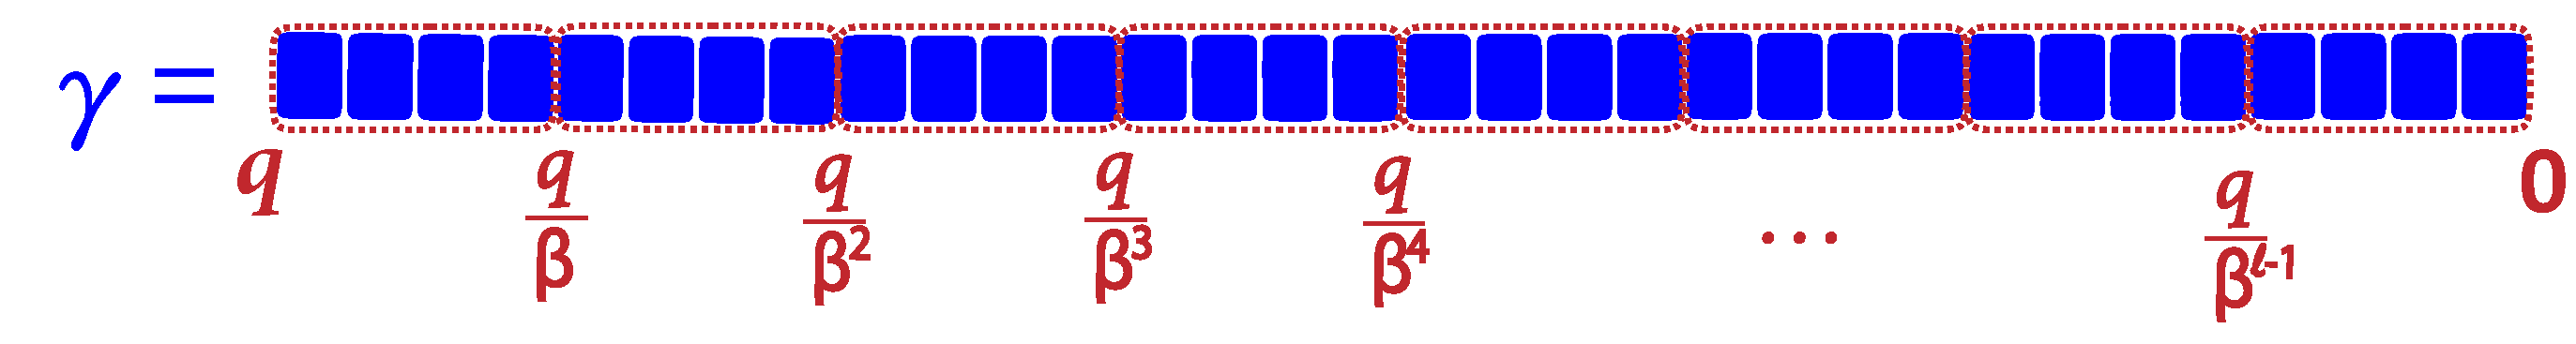
\includegraphics[width=0.8\linewidth]{figures/decomp.pdf}
  \caption{An illustration of number decomposition.}
  \label{fig:decomp}
\end{figure}

We define the decomposition of number $\gamma$ into base $\beta$ with level $\ell$ as follows:


$ $

$\textsf{Decomp}^{\beta, \ell}(\gamma) = (\gamma_1, \gamma_2, \text{ } \cdots , \text{ } \gamma_\ell)$.
 
$ $

Number decomposition is also called radix decomposition, where the base $\beta$ is called a radix. 


\subsubsection{Example}

Suppose we take $\gamma=13$ in $\mathbb{Z}_{16}$. Suppose we want to decompose 13 with the base $\beta = 2$ and level $\ell = 4$. Then, 13 is decomposed as follows:

$ $

$13 = 1 \cdot \dfrac{16}{2^1} + 1 \cdot \dfrac{16}{2^2} + 0 \cdot \dfrac{16}{2^3} + 1 \cdot \dfrac{16}{2^4}$

$ $

$\textsf{Decomp}^{2, 4}(13) = (1, 1, 0, 1)$


\subsection{Polynomial Decomposition}
\label{subsec:poly-decomp}

This time, suppose we have polynomial $f$ in the polynomial ring ${\mathbb{Z}_q[x] / (x^n + 1)}$. Therefore, each coefficient $c_i$ of $f$ is an integer modulo $q$. Polynomial decomposition expresses $f$ as a sum of multiple polynomials in base $\beta$ and level $\ell$ as follows:


\begin{tcolorbox}[title={\textbf{\tboxlabel{\ref*{subsec:poly-decomp}} Polynomial Decomposition}}]

Given $f\in \mathbb{Z}_q[x]/(x^n+1)$, fix $\beta\ge 2$ and $\ell\ge 1$ with $\beta^\ell\mid q$. We write

$ $

$f=\sum_{i=1}^{\ell} f_i\,\frac{q}{\beta^i}, \qquad f_i\in \mathbb{Z}_q[x]/(x^n+1)  $

$ $

where each $f_i$ is obtained by decomposing every coefficient of $f$ in base $\beta$. If $f=\sum_j c_j x^j$ with $c_j\in\mathbb{Z}_q$, then
$c_j=\sum_{i=1}^{\ell} c_{j,i}\, \frac{q}{\beta^i}$ with $c_{j,i}\in\{0,\ldots,\beta-1\}$,
and $f_i=\sum_j c_{j,i} x^j$.
We denote the decomposition of the polynomial $f$ into the base $\beta$ with the level $\ell$ as follows:

$ $

$\textsf{Decomp}^{\beta, \ell}(f) = (f_1, f_2, \text{ } \cdots , \text{ } f_\ell)$
 $ $
\end{tcolorbox}




\subsubsection{Example}

Suppose we have the following polynomial in the polynomial ring $\mathbb{Z}_{16}[x] / (x^4 + 1)$:

$ $

$f = 6x^3 + 3x^2 + 14x + 7 \in \mathbb{Z}_{16}[x] / (x^4 + 1)$

$ $

Suppose we want to decompose the above polynomial with base $\beta = 4$ and level $\ell = 2$. Then, each degree's coefficient of the polynomial $f$ is decomposed as follows:

$ $

${\bm{x}^{\bm{3}}}$: $6 = \color{blue}{1 \cdot \dfrac{16}{4^1}} \color{black}+ \color{red}{2 \cdot \dfrac{16}{4^2}}$

${\bm{x}^{\bm{2}}}$: $3 = \color{blue}{0 \cdot \dfrac{16}{4^1}} \color{black}+ \color{red}{3 \cdot \dfrac{16}{4^2}}$

${\bm{x}^{\bm{1}}}$: $14 = \color{blue}{3 \cdot \dfrac{16}{4^1}} \color{black}+ \color{red}{2 \cdot \dfrac{16}{4^2}}$

${\bm{x}^{\bm{0}}}$: $7 = \color{blue}{1 \cdot \dfrac{16}{4^1}} \color{black}+ \color{red}{3 \cdot \dfrac{16}{4^2}}$

$ $

The decomposed polynomial is as follows:

$f = 6x^3 + 3x^2 + 14x + 7 = \color{blue}{(1x^3 + 0x^2 + 3x + 1) \cdot \dfrac{16}{4^1}} \color{black}+ \color{red}{(2x^3 + 3x^2 + 2x + 3) \cdot \dfrac{16}{4^2}} \color{black}$

$ $

$\textsf{Decomp}^{4, 2}(6x^3 + 3x^2 + 14x + 7) = (1x^3 + 0x^2 + 3x + 1, 2x^3 + 3x^2 + 2x + 3)$

\subsubsection{Discussion}

Note that after decomposition, the original coefficients of the polynomial got reduced to smaller numbers. This characteristic is importantly used in homomorphic encryption's multiplication, for reducing the growth rate of the noise. Normally, the polynomial coefficients of ciphertexts are large because they are uniformly random numbers. Reducing such big constants is important to reduce the noise growth during homomorphic multiplication. We will discuss this more in detail in \autoref{subsec:tfhe-mult-cipher}.


\subsection{Approximate Decomposition}
\label{subsec:approx-decomp}

\begin{figure}[h!]
    \centering
  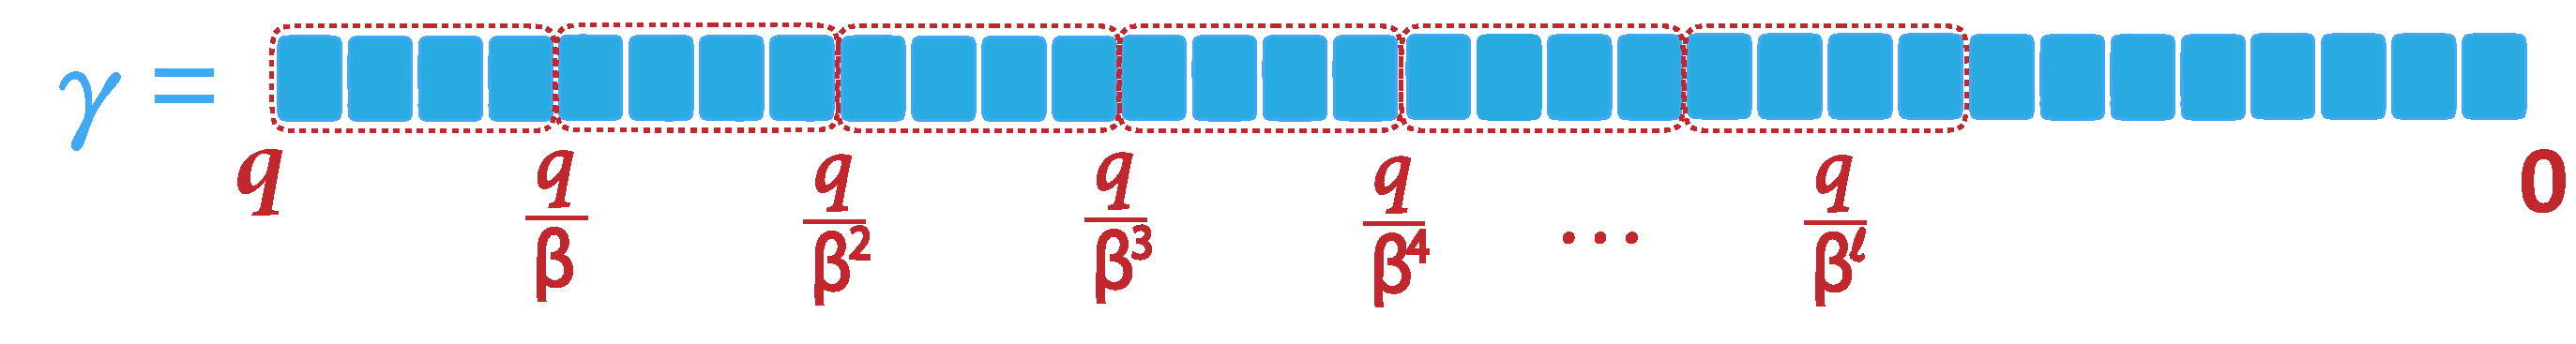
\includegraphics[width=0.7\linewidth]{figures/decomp3.pdf}
  \caption{An illustration of approximate decomposition}
  \label{fig:decomp3}
\end{figure}

If no level $\ell$ satisfies $\beta^\ell \mid q$, then some lower bits of $q$ must be discarded during decomposition, as shown in \autoref{fig:decomp3}. Such lower bits can be rounded to the nearest multiple of $\dfrac{q}{\beta^\ell}$ during decomposition. In such a case, the decomposition is an approximate decomposition. 
Formally, when $\beta^\ell\nmid q$ we can write
$$
\gamma=\sum_{i=1}^{\ell}\gamma_i\,\frac{q}{\beta^{i}}+\varepsilon,\qquad
\gamma_i\in\{0,\ldots,\beta-1\},\quad
|\varepsilon|\le \frac{q}{2\beta^{\ell}}
$$
(using nearest-integer rounding and identifying $\gamma$ with its integer representative). The polynomial case is analogous, coefficient-wise.



\subsection{Gadget Decomposition}
\label{subsec:gadget-decomposition}

Gadget decomposition is a generalized form of number decomposition (\autoref{subsec:number-decomp}). In number decomposition, a number $\gamma$ is decomposed as follows: 

$\gamma = \gamma_1 \dfrac{q}{\beta^1} + \gamma_2 \dfrac{q}{\beta^2} + \cdots + \gamma_\ell \dfrac{q}{\beta^\ell} $

$ $

In gadget decomposition, we decompose $\gamma$ as follows: 

$\gamma = \gamma_1 g_1 + \gamma_2 g_2 + \cdots + \gamma_\ell g_\ell $

$ $

We denote $\vec{g} = (g_1, g_2, \cdots, g_\ell)$ as a gadget vector, and $\textsf{Decomp}^{\vec{g}}(\gamma) = (\gamma_1, \gamma_2, \text{ } \cdots , \text{ } \gamma_\ell) $

$ $

Then, $\gamma = \langle \textsf{Decomp}^{\vec{g}}(\gamma), \vec{g} \rangle $

$ $

In the case of number decomposition (\autoref{subsec:number-decomp}), its gadget vector is $\vec{g} = \Bigg(\dfrac{q}{\beta}, \dfrac{q}{\beta^2}, \cdots, \dfrac{q}{\beta^\ell}\Bigg)$.


\clearpage

\section{Roots of Unity}
\label{sec:roots}
\textbf{- Reference:} 
\href{https://e.math.cornell.edu/people/belk/numbertheory/CyclotomicPolynomials.pdf}{Fields and Cyclotomic Polynomials}~\cite{cyclotomic-polynomial}


\subsection{Definitions}
\label{subsec:roots-def}
\begin{tcolorbox}[title={\textbf{\tboxdef{\ref*{subsec:roots-def}} Definitions for Roots of Unity}}]
\begin{itemize}
\item \textbf{$\bm{n}$-th root of Unity:} A complex number $\zeta$ that satisfies the equation $\zeta^n = 1$
\item \textbf{Primitive $\bm{n}$-th Root of Unity:} Any $n$-th root of unity $\zeta$ such that $\textsf{ord}_{\mathbb{C}}(\zeta) = n$. We denote $P(n)$ as a set of primitive $n$-th root of unity. 
\end{itemize}

$ $

A primitive $n$-th root of unity is considered a \textit{generator} of all $n$ $n$-th roots of unity.
\end{tcolorbox}

\subsection{Theorems}
\label{subsec:roots-theorem}


\begin{tcolorbox}[title={\textbf{\tboxtheorem{\ref*{subsec:roots-theorem}.1} Formula for $\bm{n}$-th Root of Unity}}]
Given $\zeta^n = 1$, there exist exactly $n$ different $n$-th roots of unity: 

$ $

$\zeta = e^{2k\pi i/n} = \cos\left(\dfrac{2k\pi}{n}\right) + i\cdot\sin\left(\dfrac{2k\pi}{n}\right)$, 

$ $

\noindent for $n$ different $k$ values, where $k = \{0, 1, \cdots, n-1\}$.
\end{tcolorbox}
\begin{myproof} 
    \begin{enumerate}
    \item Suppose $\zeta = e^{2k\pi i/n}$. Then, $\zeta^n = (e^{2k\pi i/n})^n = e^{2k\pi i}$, and since $\zeta^n = 1$, we need to find the $k$ values such that $e^{2k\pi i} = 1$
    \item Euler's formula states that $e^{i\cdot x} = \text{cos}(x) + i \cdot \text{sin}(x)$. Therefore, if $x = 2k\pi$, then $e^{2k\pi i} = \text{cos}(2k\pi) + i \cdot \text{sin}(2k\pi)$. This formula becomes 1 if $k = 0, 1, 2, ...$. Thus, $e^{2k\pi i} = 1$ for any integer $k \geq 0$. 
    \item If $\zeta = e^{2k\pi i/n} = \text{cos}(\frac{2k\pi}{n}) + i\cdot\text{sin}(\frac{2k\pi}{n})$, then the first $n$ roots for $k = 0, 1, ... \text{ } n-1$ are all distinct values, because they lie on the circle in the complex plane (where $x$-axis is a real value and $y$-axis is a complex value coefficient) at each angle $2k\pi/n$ for $k = \{0, 1, \cdots, n-1\}$.
    \item Note $\zeta^n = 1$ is an $n$-th polynomial, so it can have at most $n$ roots. Thus, we can consider the first $n$ roots $e^{2k\pi i/n}$ for $k = \{0, 1, \cdots, n-1\}$ as the $n$ distinct roots and ignore the rest of roots (i.e., $k \geq n$), considering them to be repetitions of the first $n$ roots on a circle in the complex plane (see \autoref{fig:complex-plane}). 
    \end{enumerate}
\end{myproof}

\begin{figure}[h!]
    \centering
  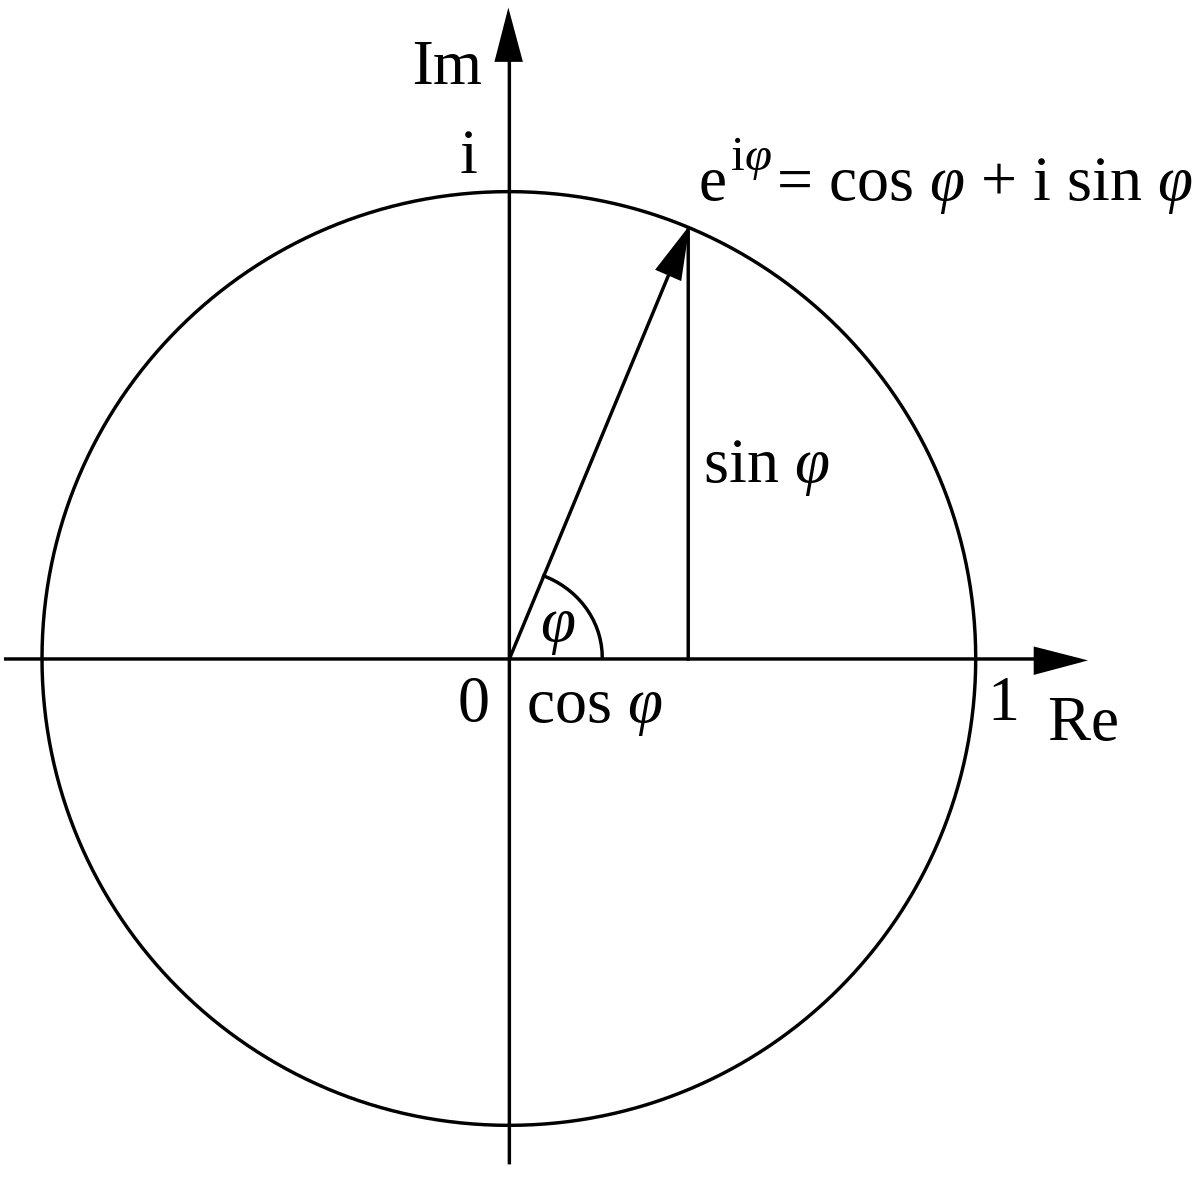
\includegraphics[width=0.4\linewidth]{figures/euler-formula.png}
  \caption{The figure illustrates a circle of Euler's formula in the complex plane \href{https://en.wikipedia.org/wiki/Euler's_formula}{(Source)}}
  \label{fig:complex-plane}
\end{figure}


\begin{tcolorbox}[title={\textbf{\tboxtheorem{\ref*{subsec:roots-theorem}.2} Order of the Root of Unity}}]
Given $\zeta \in \mathbb{C}$ (the complex number domain) and $\zeta^n = 1$ where $n \geq 1$, $\zeta$ is an $n$-th root of unity if and only if $\textsf{ord}_{\mathbb{C}}(\zeta) \text{ } | \text{ } n$.
\end{tcolorbox}
\begin{proof}
    We use 
    Theorem~\ref*{subsec:order-theorem}.1:
    \begin{enumerate}
    \item \textit{Forward Proof:} Since $\textsf{ord}_{\mathbb{C}}(\zeta)=k$ is the smallest integer such that $\zeta^k = 1$, for any $n$ that satisfies $\zeta^n = 1$, $n$ must be a multiple of $k$. This means that $k \gap{$|$} n$.
    \item \textit{Backward Proof:} If $k \gap{$|$} n$, then $n$ is a multiple of $k$, which means that $\zeta^n = 1$. 
    \end{enumerate}
    %$(Here, note that our \b\bmodulo computation wraps around a circle of Euler's formula on the complex plane instead of a finite integer field).
\end{proof}

\begin{tcolorbox}[title={\textbf{\tboxtheorem{\ref*{subsec:roots-theorem}.3} Set of All $\bm{n}$-th Roots of Unity}}]
The set of all $n$-th roots of unity is the union $\bigcup_{d|n} P(d)$ (i.e., the union of all primitive $d$-th roots of unity where $d \text{ } | \text{ } n$).
\end{tcolorbox}
\begin{myproof}
    \begin{enumerate}
    \item Let $\omega = e^{2\pi i/n}$.
    Given $\zeta^n = 1$, for each $n$-th root of unity $\zeta$ is, $\zeta = \omega^{k_i}$ for $k_i = \{0, 1, \cdots, n-1\}$. Note that according to Theorem~\ref*{subsec:order-theorem}.1, $(\omega^{k_i})^n = 1$ if and only if $\textsf{ord}_{\mathbb{C}}(\omega^{k_i}) \text{ } | \text{ } n$. 
    \item Let $\textsf{ord}_{\mathbb{C}}(\omega^{k_i}) = d_i$. Then, $(\omega^{k_i})^{d_i} = 1$. Combining these two facts, each $n$-th root of unity $\omega^{k_i}$ is also a primary $d_i$-th root of unity (i.e., a solution for $\zeta^{d_i} = 1$), that is, $\omega^{k_i} \in P(d_i)$. 
    \item Remember that for each $\textsf{ord}_{\mathbb{F}}(\omega^{k_i}) = d_i$, $d_i \text{ } | \text{ } n$. For every $d_i$ that divides $n$, all the (primary) $d_i$-th roots of unity are also the $n$-th root of unity. This is because the (primary) $d_i$-th root of unity that satisfies $\zeta^{d_i} = 1$ also satisfies $\zeta^{n} = 1$ (as $n$ is a multiple of $d_i$).
    \item Step 2 concludes that each $n$-th root of unity is a primitive $d_i$-th root of unity for some $d_i$ that divides $n$. Step 3 concludes that each $d_i$-th root of unity, where $d_i$ divides $n$, is also the $n$-th root of unity. Combining these two conclusions, the set of all primitive $n$-th root of unity is equivalent to the union of all primary $d_i$-th roots of unity where $d_i$ divides $n$ (i.e., $\bigcup_{d|n} P(d)$). 
    \end{enumerate}
\end{myproof}

\begin{tcolorbox}[title={\textbf{\tboxtheorem{\ref*{subsec:roots-theorem}.4} Condition for Primitive $\bm{n}$-th Roots of Unity}}]
Given an $n$-th root of unity $\zeta = \omega^k$ for $k = \{0, 1, \cdots, n-1\}$ where $\omega = e^{2\pi i/n}$, $\zeta$ is a primitive $n$-th root of unity if and only if $\text{gcd}(n, k) = 1$ (i.e., $k$ is co-prime to $n$).
\end{tcolorbox}
\begin{myproof}
    \begin{enumerate}
    \item Note that $\zeta^n = 1$ and $\zeta = \omega$ for $k = 1$. Thus, $\textsf{ord}_{\mathbb{C}}(\omega) = n$.
    \item Theorem~\ref*{subsec:order-theorem}.2 states that if $ord_{\mathbb{F}}(a) = k$, then for any $n \geq 1$, $ord_{\mathbb{F}}(a^n) = \dfrac{k}{\text{gcd}(k,n)}$. Similarly, if $\textsf{ord}_{\mathbb{C}}(\omega) = n$, then for any $k \geq 1$, $\textsf{ord}_{\mathbb{C}}(\omega^k) = \dfrac{n}{\text{gcd}(k, n)}$.
    \item Step 2 implies that $\textsf{ord}_{\mathbb{C}}(\omega^k) = n$ (i.e., $\omega^k$ is a primitive $n$-th root of unity) if and only if $\text{gcd}(k, n) = 1$.
    \end{enumerate}
\end{myproof}

\begin{tcolorbox}[title={\textbf{\tboxtheorem{\ref*{subsec:roots-theorem}.5} The number of Primitive $\bm{n}$-th Roots of Unity}}]
The number of primitive $n$-th roots of unity is $\phi(n)$ (i.e., the number of elements in $\{1, \cdots, n-1 \}$ that are coprime to $n$).
\end{tcolorbox}

\begin{proof}
$ $
\begin{enumerate}
\item Given $\zeta^n = 1$, the roots of unity are $\zeta = \omega^k$ where $\omega = e^{2\pi i/n}$ and $k = \{0, 1, \cdots, n-1\}$ 
\item By definition, $\omega^k$ is a primitive $n$-th root of unity if and only if $\textsf{ord}_{\mathbb{C}}(\omega^k) = n$. 
\item $\omega$ is a primitive $n$-th root of unity, because $\textsf{ord}_{\mathbb{C}}(\omega) = n$. 
\item According to Theorem~\ref*{subsec:order-theorem}.2, if $\textsf{ord}_{\mathbb{C}}(\omega) = n$, then $\textsf{ord}_{\mathbb{C}}(\omega^k) = \dfrac{n}{\text{gcd}(k,n)}$. Therefore, in order for $\textsf{ord}_{\mathbb{C}}(\omega^k) = n$, $\text{gcd}(k,n)$ has to be 1. In other words, $k$ and $n$ have to be co-prime.
The total number of such co-primes between $n$ and $k = \{1, 2, \cdots, n-1\}$ (excluding 0 because $\text{gcd}(0, n)= n$ and also $\textsf{ord}_{\mathbb{C}}(\omega^0) = \textsf{ord}_{\mathbb{C}}(1) = 1 \neq n$) is $\phi(n)$, which corresponds to the total number of the primitive $n$-the root of unity.
\end{enumerate}
\end{proof}

\clearpage




\bibliographystyle{unsrt}
\bibliography{z-bibfile}



%\clearpage
%\input{scratch-real}

\end{document}


%https://www.youtube.com/watch?v=vYKdh5oQ4Zw
